\section{Defects and noises} \label{sec:defects}

There are various ways the CCD image can be distorted or corrupted and also numerous sources of these defects. 


\subsection{Statistical noise}

    %%%%%%%%%%%%%%%%%%%%%%%%%%%% 
    \subsubsection{Photon noise}
    
    The distribution of photons falling on the CCD chip obeys simple counting statistics. 
    Let's assume the CCD chip is illuminated with constant uniform light and that the sensitivity of each pixel is the same. 
    For each finite moment, there is an amount of photons detected on the chip which varies.
    If we were to plot the amount of photons detected and the occurrences of each amount in a histogram, we would quickly realise that the distribution is following a Poisson distribution. As we are dealing with large amount of photons, Poisson distribution can be approximated with the Gaussian function: 
    
    \begin{equation}
     \label{eqn:gaussian}
        g(x) = \frac{1}{\sigma \cdot \sqrt{2 \pi}} \cdot exp \left(  - \frac{1}{2} \cdot \frac{(x - \mu)^2}{\sigma^2} \right)   
    \end{equation}
    
    where $\mu$ is the average or the most common amount of photons detected and $\sigma$ is the standard deviation. 
    The number of photons detected on the chip can also be referred to as a signal $S$ \cite{romanishin2006introduction}.
    
    Let's denote, that $S_{star}$ is the signal from the star and $S_{sky}$ is the signal from the sky. From \cite{romanishin2006introduction} the noise from the star $\sigma_{star}$ and the noise from the sky $\sigma_{sky}$ can be expressed as:
    
    \begin{equation}
    \label{eqn:starskynoise}
        \sigma_{star} = \sqrt{S_{star}} \quad \sigma_{sky} = \sqrt{S_{sky}}
    \end{equation} 

    and addition of these noises is done in a following manner:
    \begin{equation}
    \label{eqn:additionNoises}
        \sigma = \sqrt{\sigma_{star}^2 + \sigma_{sky}^2}
    \end{equation}

\subsection{Internal}

Internal defects and noises are caused by issues within the CCD chip. This includes mechanical and electrical issues. 
 

    %%%%%%%%%%%%%%%%%%%%%%%%%%%% 
    \subsubsection{Bias}
    
    In the process of accumulating photo-electrons in the CCD chip, let's suppose that each pixel accumulated 2 photo-electrons on average. Given how the analog to digital conversion works, a number of counts $N_{counts}$ is proportional to a number of photo-electrons $N_{elec}$ accumulated in the pixel and is expressed by the following: 
        
    \begin{equation}
    \label{eqn:bias}
        N_{elec}  = gain \cdot N_{counts}
    \end{equation}
    
    For the simplicity of the example let's suppose that the gain is 1 e-/ADU. According to the formula, each pixel should have 2 counts, but due to the readout noise, the number of counts will follow the Gaussian distribution. The mean of the Gaussian is 2 counts, with a standard deviation given by the readout noise, which could be as much as 3 counts. This would mean that the number of counts in some pixels would be negative. However, the ADC cannot represent negative numbers, which means that the data would be corrupted \cite{articleCCDartifacts} \cite{phy217}.
    To fix this issue, bias voltage was applied to the CCD detector. It is a constant offset voltage, which means that even if the pixel contained no photo-electrons, the ADC returns a high positive value. This solves the issue with negative values. The constant bias voltage is identified through the BIAS frame \cite{articleCCDartifacts} \cite{phy217}.
    
        
 
    %%%%%%%%%%%%%%%%%%%%%%%%%%%% 
    \subsubsection{Readout noise}
    
    Reading out the image from the CCD chip includes charge shifting through the chip followed by conversion to the voltage. Due to the limitations in the current technology, the voltage in the pixel cannot be measured perfectly and readout noise is introduced. 
    The noise is expressed as the number of electrons per pixel. This number is characteristic for each CCD chip and is usually defined by manufacturers.
    Readout noise is generated during the process of reading the image, therefore it is independent of the exposure time of the image. However, the amount of noise increases with the higher speed of the readout \cite{articleCcdOnline}.
    
    From \cite{bolte15} readout noise in the aperture can be expressed as: 
    
    \begin{equation}
    \label{eqn:readoutNoise}
         \sigma_{RN} = \sqrt{N_{pix} \cdot {RN}^2 }
    \end{equation}
    
    where $N_{pix}$ is a number of pixels in the aperture and $RN$ is readout noise in electrons per pixel.

    Note, that the readout noise is not following Poisson distribution and is not related to the signal coming from stars or sky \cite{matfyzpress01}. Therefore Formula \ref{eqn:starskynoise} cannot be used, when expressing the readout noise. 

    %%%%%%%%%%%%%%%%%%%%%%%%%%%% 
    \subsubsection{Dark current}
    
    Photo-electrons in CCD pixels are produced by photons from incoming light. However, thermal excitation can also produce electrons in pixels, and it's impossible to differentiate between them and photo-electrons coming from the light \cite{phy217}.
    This effect is called dark current and is expressed in electrons per second per pixel at the defined temperature. The amount of dark current is linearly proportional to chip temperature and exposure time. To minimize the effect, CCD chips are usually cooled down to a temperature below 0°C \cite{articleCcdOnline}.
    
    The amount of dark current is also affected by pixel size, chip architecture, and production technology. Therefore manufacturers usually define the amount of dark current for specific models of CCD chips.
    Even after the chip is cooled, the amount of dark current is not negligible. To detect the dark current in the image, DARK frames were created \cite{articleCcdOnline}. The noise from the dark current is also following Poisson distribution \cite{matfyzpress01}. 
    
    From \cite{bolte15} the noise caused by dark current in our aperture can be expressed as:
    
    \begin{equation}
    \label{eqn:darkcurrent}
        \sigma_{DC} = \sqrt{D \cdot N_{pix} \cdot t}
    \end{equation}

    
    where $D$ is dark current in $e^-/second/pixel$, $N_{pix}$ is number of pixels in the aperture and $t$ is the exposure time.
    
    
    \begin{figure}[!h]
    \centering
        \begin{subfigure}{.3\textwidth}
        \centering
            
\includegraphics[width=\textwidth]{images/hotpixels.png}
            \caption{Hot pixels.}
            \label{fig:hotpixels}
        \end{subfigure}
        \begin{subfigure}{.3\textwidth}
            \centering
            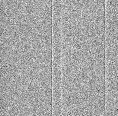
\includegraphics[width=\textwidth]{images/deadcolumns.jpg}
            \caption{Dead columns.}
            \label{fig:deadcolumns}
        \end{subfigure}
        
        \vspace*{4mm}
        
        \begin{subfigure}{.3\textwidth}
            \centering
            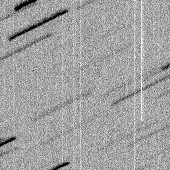
\includegraphics[width=\textwidth]{images/traps2.jpg}
            \caption{Traps.}
            \label{fig:trap}
        \end{subfigure}
        \begin{subfigure}{.3\textwidth}
            \centering
            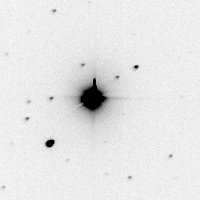
\includegraphics[width=\textwidth]{images/saturationtrail.png}
            \caption{Saturation trail.}
            \label{fig:saturationtrail}
        \end{subfigure}
        \caption{Examples of some internal defects present on FITS images acquired by AGO70.}
        \label{fig:internaldefects}
    \end{figure}
    
    
    
    
    
    %%%%%%%%%%%%%%%%%%%%%%%%%%%% 
    \subsubsection{Hot Pixels}
    
    Hot pixels (Figure \ref{fig:hotpixels}) are individual pixels that have a very high dark current, meaning they are really bright or fully saturated. This is related to the defect of the chip which was either created during the manufacturing or by aging. Fully saturated pixels have reached their limit of detected photo-electrons, which means that any incoming photons will not generate any electrons. 
    As this is the result of the CCD chip issue, their positions on the image are fixed. This makes them easy to detect on a DARK frame.
    % citacia

        
    %%%%%%%%%%%%%%%%%%%%%%%%%%%% 
    \subsubsection{Dead Pixels}
    
    Dead pixels are also individual pixels, which on the contrary are not sensitive to any light and are completely dark. Similar to hot pixels, their positions are fixed from image to image and can be detected on the DARK frame.
    % citacia
    
    %%%%%%%%%%%%%%%%%%%%%%%%%%%% 
    \subsubsection{Dead columns} 
    
    Dead columns (Figure \ref{fig:deadcolumns})are columns of pixels corrupted in some way. %as depicted in the figure \ref{fig:deadcolumns}. 
    They can be either completely dark (not sensitive to any incoming photons) or fully saturated (reached the limit of detected photo-electrons). Apart from that, dead columns can also have a constant value added to what their real value should be. 
    They are various reasons for this defect, mechanical or electronical \cite{articleCCDartifacts}.
    
    
    
    %%%%%%%%%%%%%%%%%%%%%%%%%%%% 
    \subsubsection{Traps} 
    
    Traps (Figure \ref{fig:trap}) occur when some pixels on the CCD chip are damaged in a way that they cannot transfer photo-electrons \cite{articleCCDartifacts}. 
    As mentioned earlier during the process of reading the image, the charge is shifted through pixels. All rows are shifted one row below and the last row is shifted to the horizontal register from which the charge is shifted to the ADC \cite{articleCcdOnline}. However, if a pixel is damaged, the charge cannot pass through during the shifting of the rows. 
    
    Let's assume, the damaged pixel is in the first column and on the 4th-row counting from the top. Note that damage is only present in the first column, which contained the damaged pixel and other columns are unaffected.
    
    Pixels below the 4th row are read normally. However, pixels in the first three rows cannot be shifted through the damaged 4th pixel. Electrons in these pixels are therefore trapped and their charge cannot be converted to counts. This will result in completely dark pixels in these first three rows. %An example of a vertical trap is shown in the figure \ref{fig:trap} 
    
    Note, that traps are vertical when the CCD chip is read horizontally, by shifting charge from one row to another. However, in case the chip is read vertically and the charge is shifting through columns, traps will be horizontal. 


    %%%%%%%%%%%%%%%%%%%%%%%%%%%%
    \subsubsection{Saturation trail}
    
    Each pixel on the CCD chip has a certain amount of photo-electrons it can store. Some very bright sources can illuminate pixels to the point where they are completely filled up. As the pixel is filled to its limit, photo-electrons from the saturated pixel can start leaking to adjacent pixels. These extra electrons create a trail of saturated pixels - saturation trail (Figure \ref{fig:saturationtrail}) \cite{articleCCDartifacts}.
    
    Similar to traps, trails are either horizontal or vertical and it depends on the way the CCD chip is read. 
    



\subsection{External}

External noises and defects are caused by external forces such as moonlight, sunlight, particles in the universe, the atmosphere, and many others. All these effects are discussed below.

    
    %%%%%%%%%%%%%%%%%%%%%%%%%%%% 
    \subsubsection{Sky background noise} 
    
    One of the most dominant sources of noise in CCD images is the noise from the sky. This is caused by various sources of light present in the sky as well as some photons flying through space. 
    %For stars to be seen, their signal must be brighter than the noise coming from the sky. However, this does not mean that fainter stars will never be seen. The amount of signal is not as important as the ratio of the signal to the current noise in the sky. As this is a common problem in astronomy, this ratio is well known and is called signal-to-noise ratio - SNR. The higher the ratio, the easier it is to see the signal from the stars.
    The sky noise is not constant and changes depending on various circumstances. As the sky gets brighter, the noise from the sky increases as well. This is caused by light pollution. Decreasing noise can be therefore observed when the sky is the darkest. Since the signal from stars has a constant value and the noise has a decreasing tendency this results in higher SNR of star signals \cite{romanishin2006introduction}. 
    
    Sky observations are usually done when the sky is darkest and at remote places to avoid light pollution. However even this does not guarantee the perfect dark sky. Various atomic processes are happening in the atmosphere. Molecules and atoms are constantly colliding with each other, which causes the excitation of atoms. This causes the air to glow which is yet another source of light contributing to the sky background noise. 
    In the case of space-based observations, the sky is darker compared to observations from Earth as there is no light coming from artificial sources and the atmosphere. However, another dominant source of light is present, which is called zodiacal light. This is sunlight scattered by dust particles and is present in the whole Solar system \cite{romanishin2006introduction}.
    
    %With low exposure time, the amount of sky noise is also very low and electronic noises are dominating the overall noise.
    
    %%%%%%%%%%%%%%%%%%%%%%%%%%%% 
    \subsubsection{Stray light} 

    Stray light (Figure \ref{fig:straylight})is caused by the reflection of light from optical surfaces like tubes or domes. Various sources of light can be reflected. This includes scattered moonlight which causes a bright gradient present in the image. Artificial sources of light such as diodes or internal lights can also be reflected on the image.
    % citacia
    
    %%%%%%%%%%%%%%%%%%%%%%%%%%%% 
    \subsubsection{Diffuse sources} 
    
    Diffuse sources such as galaxies (Figure \ref{fig:diffgalaxy}), nebulas, and comets (Figure \ref{fig:comet}) are also contributing to image corruption. They are not explicitly defects or noises, but their presence in the image can cause problems during photometry as they are contributing to the sky‘s brightness. 

        
    %%%%%%%%%%%%%%%%%%%%%%%%%%%%
    \subsubsection{Dust on filter}
    
    Dust particles (Figure \ref{fig:dust}) present on the lens or filters of the aperture can also cause problems in the image. Apart from other defects mentioned, which are usually only locally on the image, dust particles affect the image globally. The particles cast shadows on the detector and this manifests on the image in a form of dark rings \cite{articleCCDartifacts}.
    FLAT FIELD frame can detect these defects and thus are later corrected in a photometric reduction \cite{articleParimucha}.
    
    
    \begin{figure}[!h]
    \centering
        \begin{subfigure}{.3\textwidth}
        \centering
            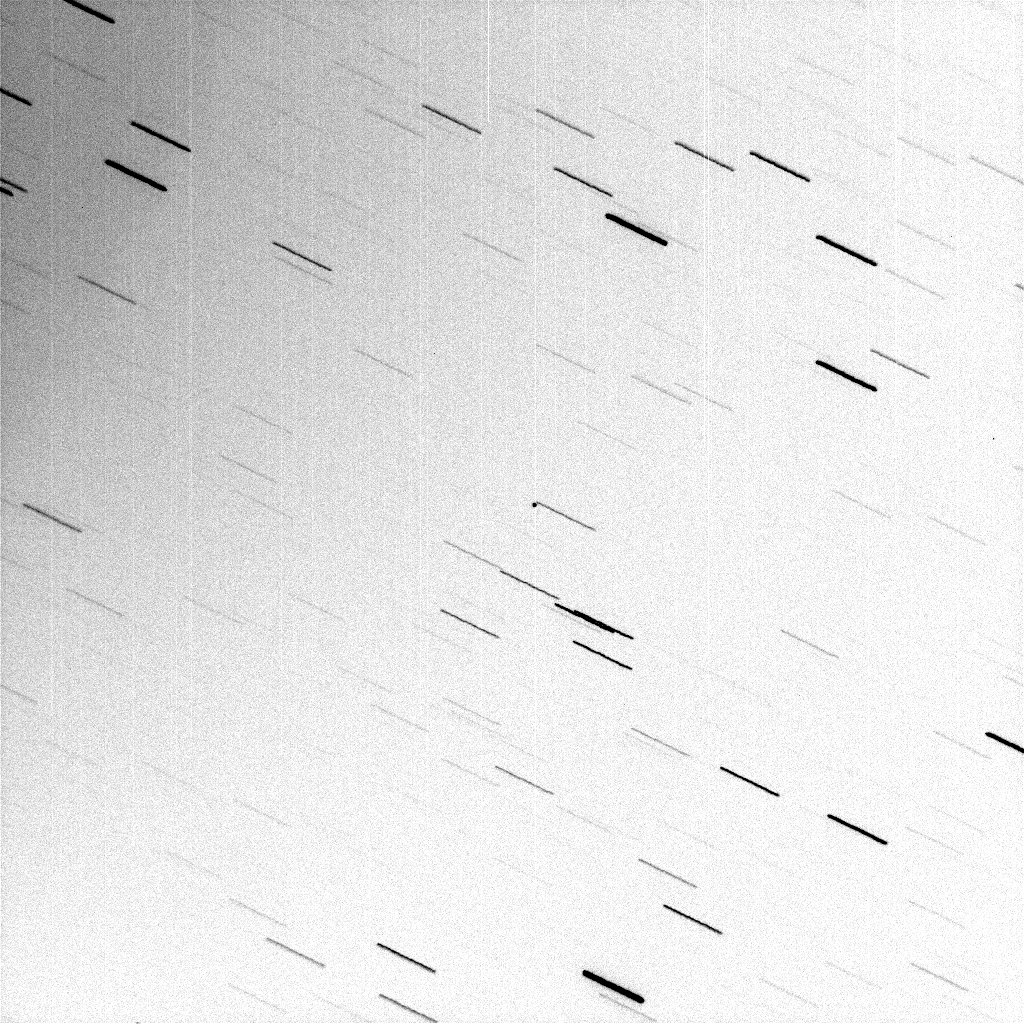
\includegraphics[width=\textwidth]{images/straylight.png}
            \caption{Stray light.}
            \label{fig:straylight}
        \end{subfigure}
        \begin{subfigure}{.3\textwidth}
            \centering
            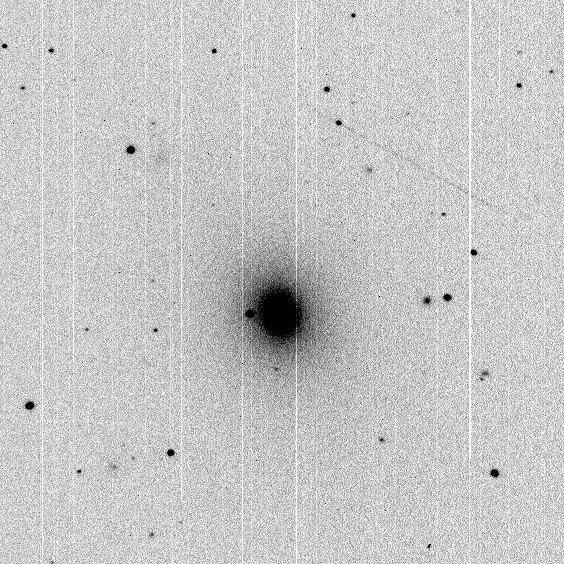
\includegraphics[width=\textwidth]{images/galaxyreal.jpg}
            \caption{Galaxy.}
            \label{fig:diffgalaxy}
        \end{subfigure}

        \vspace*{4mm}

        \begin{subfigure}{.3\textwidth}
            \centering
            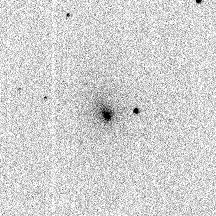
\includegraphics[width=\textwidth]{images/comet.jpg}
            \caption{Comet.}
            \label{fig:comet}
        \end{subfigure}
        \begin{subfigure}{.3\textwidth}
            \centering
            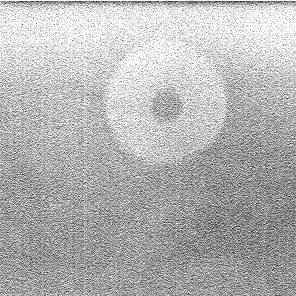
\includegraphics[width=\textwidth]{images/dust.jpg}
            \caption{Dust ring.}
            \label{fig:dust}
        \end{subfigure}
        \caption{Examples of some external defects present on FITS images acquired by AGO70.}
        \label{fig:externaldefects}
    \end{figure}
 
    %%%%%%%%%%%%%%%%%%%%%%%%%%%% 
    \subsubsection{Cosmic rays}
    
    %A CCD chip is an instrument detecting photons emitting from light sources. Each photon creates a single electron in a specific pixel of the chip. 
    Flying through space are also high-energy particles called cosmic rays.  Each particle can excite hundreds or thousands of electrons, which can also cross through multiple pixels. 
    A cosmic ray hitting the CCD chip is an unpredictable event that can occur randomly affecting the image locally \cite{imageProc}. The temperature of the chip or its defects do not affect the event of cosmic rays hitting the chip. However, the longer the exposition time, the more cosmic rays hit the chip. 
    Cosmic rays can manifest as a single very bright pixel but sometimes it affects several adjacent pixels. The created object has strong and asymmetric features with sharp edges \cite{irafArticle}.
    
    Their profile can be classified into three categories \cite{inbookCosmics} which are shown in the Figure \ref{img:cosmicraysreal}  
        \begin{itemize}
            \item spot-like - resemble dots
            \item track-like - resemble straight lines
            \item worm-like - resemble polylines and curves
        \end{itemize}
    
    
    They could also be described as a group of connected pixels, which have count values higher than the background and at least one pixel having a significantly high value \cite{inbookCosmics}.
    
    When it comes to ground-based observations, they don't suffer from cosmic rays as much as space-based. Mainly because the amount of cosmic rays significantly increases in space. 

    \begin{figure}[!h]
    \centering
        
        \begin{subfigure}{\textwidth}
            \centering
            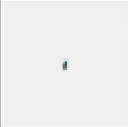
\includegraphics[width=.13\textwidth]{images/spot1.png}
            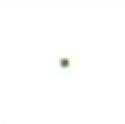
\includegraphics[width=.13\textwidth]{images/spot2.png}
            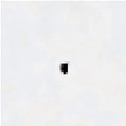
\includegraphics[width=.13\textwidth]{images/spot3.png}
            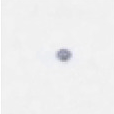
\includegraphics[width=.13\textwidth]{images/spot4.png}
            \caption{Spots.}
        \end{subfigure}
        \vskip\baselineskip
        \begin{subfigure}{\textwidth}
            \centering
            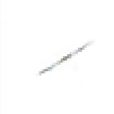
\includegraphics[width=.13\textwidth]{images/track1.png}
            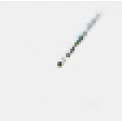
\includegraphics[width=.13\textwidth]{images/track2.png}
            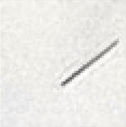
\includegraphics[width=.13\textwidth]{images/track3.png}
            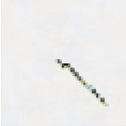
\includegraphics[width=.13\textwidth]{images/track4.png}
            \caption{Tracks.}
        \end{subfigure}
        \vskip\baselineskip
        \begin{subfigure}{\textwidth}
            \centering
            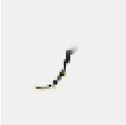
\includegraphics[width=.13\textwidth]{images/worm1.png}
            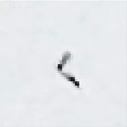
\includegraphics[width=.13\textwidth]{images/worm2.png}
            
\includegraphics[width=.13\textwidth]{images/worm3.png}
            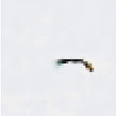
\includegraphics[width=.13\textwidth]{images/worm4.png}
            \caption{Worms.}
        \end{subfigure}
        
        \caption{Examples of three categories of cosmic rays. Source \cite{cosmicrayimageall}.}
        \label{img:cosmicraysreal}  
    \end{figure}